\documentclass[8pt,aspectratio=169]{beamer}
\usetheme{Madrid}
\usepackage{graphicx,booktabs,adjustbox,multicol,amsmath,amssymb,listings,xcolor,colortbl}
\definecolor{mlblue}{RGB}{0,102,204}
\definecolor{mlpurple}{RGB}{51,51,178}
\definecolor{mllavender}{RGB}{173,173,224}
\definecolor{mllavender2}{RGB}{193,193,232}
\definecolor{mllavender3}{RGB}{204,204,235}
\definecolor{mllavender4}{RGB}{214,214,239}
\definecolor{mlorange}{RGB}{255,127,14}
\definecolor{mlgreen}{RGB}{44,160,44}
\definecolor{mlred}{RGB}{214,39,40}
\definecolor{mlgray}{RGB}{127,127,127}
% Solidity colors
\definecolor{solkeyword}{RGB}{0,102,153}
\definecolor{solstring}{RGB}{163,21,21}
\definecolor{solcomment}{RGB}{0,128,0}
\definecolor{solnumber}{RGB}{0,128,128}
\setbeamercolor{palette primary}{bg=mllavender3,fg=mlpurple}
\setbeamercolor{palette secondary}{bg=mllavender2,fg=mlpurple}
\setbeamercolor{palette tertiary}{bg=mllavender,fg=white}
\setbeamercolor{palette quaternary}{bg=mlpurple,fg=white}
\setbeamercolor{structure}{fg=mlpurple}
\setbeamercolor{title}{fg=mlpurple}
\setbeamercolor{frametitle}{fg=mlpurple,bg=mllavender3}
\setbeamercolor{block title}{bg=mllavender2,fg=mlpurple}
\setbeamercolor{block body}{bg=mllavender4,fg=black}
\setbeamertemplate{navigation symbols}{}
\setbeamertemplate{itemize items}[circle]
\setbeamersize{text margin left=5mm,text margin right=5mm}
\newcommand{\bottomnote}[1]{\vfill\vspace{-2mm}\textcolor{mllavender2}{\rule{\textwidth}{0.4pt}}\par\vspace{1mm}\footnotesize\textbf{#1}}
% Solidity language definition
\lstdefinelanguage{Solidity}{
  keywords={pragma, solidity, contract, function, public, private, external, internal, view, pure, payable, returns, return, if, else, for, while, mapping, address, uint, uint256, int, string, bool, bytes, bytes32, event, emit, modifier, require, constructor, memory, storage, calldata, msg, sender, value, this, new, delete, true, false, import, is, constant, override, virtual},
  keywordstyle=\color{solkeyword}\bfseries,
  sensitive=true,
  comment=[l]{//},
  morecomment=[s]{/*}{*/},
  commentstyle=\color{solcomment}\ttfamily,
  stringstyle=\color{solstring}\ttfamily,
  morestring=[b]',
  morestring=[b]"
}
\lstset{language=Solidity,basicstyle=\ttfamily\scriptsize,breaklines=true,frame=single,backgroundcolor=\color{mllavender4},numbers=left,numberstyle=\tiny\color{mlgray},numbersep=5pt,tabsize=2,showstringspaces=false}
\usepackage{tikz,pgfplots}
\pgfplotsset{compat=1.18}
\usetikzlibrary{arrows.meta,positioning,shapes.geometric,calc,chains,decorations.pathmorphing,automata,fit}
\title{Deploy Your Own Cryptocurrency: Hands-On Lab \& Deep Dive}
\subtitle{Standalone Technical Lab}
\author{Prof.~Dr.~Joerg Osterrieder}
\institute{University Lecture Series}
\date{\today}
\begin{document}

%% ============================================================
%% FRAME 1: TITLE
%% ============================================================
\begin{frame}[plain]
\vspace{2cm}
\begin{center}
{\Huge\color{mlpurple} Deploy Your Own Cryptocurrency}\\[0.4cm]
{\Large\color{mlblue} Hands-On ERC-20 Lab \& Deep Dive}\\[0.3cm]
{\normalsize Standalone Technical Lab}\\[0.3cm]
\textcolor{mlgray}{\rule{6cm}{0.4pt}}\\[0.3cm]
{\small\itshape ``From zero to token in 15 minutes''}\\[1.5cm]
{\normalsize Prof.~Dr.~Joerg Osterrieder}\\[0.2cm]
{\small University Lecture Series}\\[0.2cm]
{\small \today}
\end{center}
\end{frame}

%% ============================================================
%% FRAME 2: PART A SECTION DIVIDER
%% ============================================================
\begin{frame}{}
\vfill
\begin{beamercolorbox}[sep=12pt,center,rounded=true,shadow=true]{palette quaternary}
{\Large\bfseries Part 1: Deploy Your Own Cryptocurrency}\\[6pt]
{\normalsize A step-by-step hands-on lab using Remix IDE and Sepolia testnet}
\end{beamercolorbox}
\vfill
\end{frame}

%% ============================================================
%% FRAME 3: THE MISSION (Comic Strip - 3 panels)
%% ============================================================
\begin{frame}{The Mission}
\begin{center}
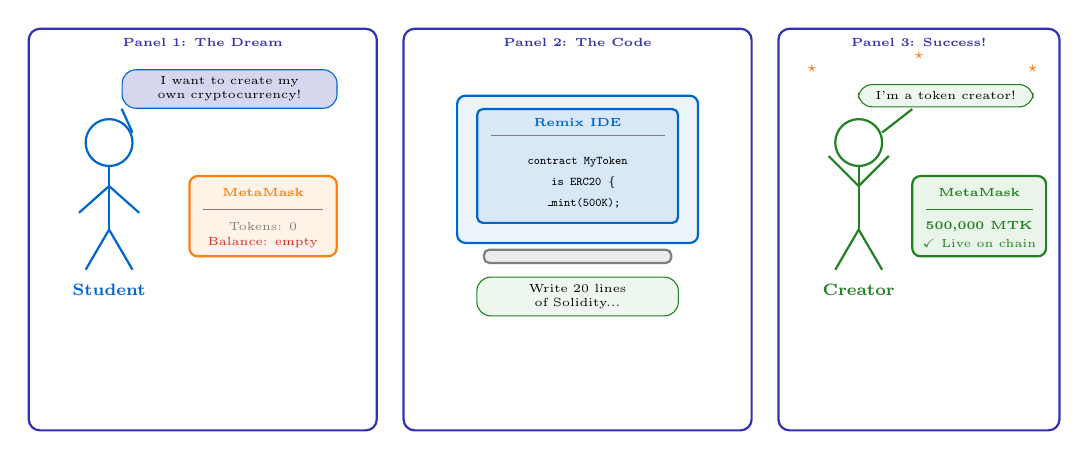
\begin{tikzpicture}[scale=0.85, every node/.style={transform shape}]

% --- Panel 1: Student with empty wallet ---
\draw[mlpurple, thick, rounded corners=4pt] (-7.2,-2.8) rectangle (-2.0,3.2);
\node[font=\tiny\bfseries, mlpurple] at (-4.6,3.0) {Panel 1: The Dream};

% Student stick figure
\draw[mlblue, thick] (-6.0,1.5) circle (0.35);
\draw[mlblue, thick] (-6.0,1.15) -- (-6.0,0.2);
\draw[mlblue, thick] (-6.0,0.85) -- (-6.45,0.45);
\draw[mlblue, thick] (-6.0,0.85) -- (-5.55,0.45);
\draw[mlblue, thick] (-6.0,0.2) -- (-6.35,-0.4);
\draw[mlblue, thick] (-6.0,0.2) -- (-5.65,-0.4);
\node[font=\scriptsize\bfseries, mlblue] at (-6.0,-0.7) {Student};

% MetaMask wallet box
\draw[mlorange, thick, fill=mlorange!10, rounded corners=3pt] (-4.8,-0.2) rectangle (-2.6,1.0);
\node[font=\tiny\bfseries, mlorange] at (-3.7,0.75) {MetaMask};
\draw[mlgray, thin] (-4.6,0.5) -- (-2.8,0.5);
\node[font=\tiny, mlgray] at (-3.7,0.25) {Tokens: 0};
\node[font=\tiny, mlred] at (-3.7,0.0) {Balance: empty};

% Speech bubble
\node[draw=mlblue, fill=mllavender4, rounded corners=5pt, font=\tiny,
      text width=3.0cm, align=center, inner sep=3pt]
      (stud-bubble) at (-4.2,2.3) {I want to create my own cryptocurrency!};
\draw[mlblue, thick] (-5.65,1.65) -- (stud-bubble.south west);

% --- Panel 2: Coding in Remix ---
\draw[mlpurple, thick, rounded corners=4pt] (-1.6,-2.8) rectangle (3.6,3.2);
\node[font=\tiny\bfseries, mlpurple] at (1.0,3.0) {Panel 2: The Code};

% Laptop / screen
\draw[mlblue, thick, fill=mlblue!8, rounded corners=3pt] (-0.8,0.0) rectangle (2.8,2.2);
\draw[mlblue, thick, fill=mlblue!15, rounded corners=2pt] (-0.5,0.3) rectangle (2.5,2.0);
\node[font=\tiny\bfseries, mlblue] at (1.0,1.8) {Remix IDE};
\draw[mlgray, thin] (-0.3,1.6) -- (2.3,1.6);
\node[font=\tiny, align=left] at (1.0,1.2) {\texttt{contract MyToken}};
\node[font=\tiny, align=left] at (1.0,0.9) {\texttt{~~is ERC20 \{}};
\node[font=\tiny, align=left] at (1.0,0.6) {\texttt{~~\_mint(500K);}};

% Speech bubble
\node[draw=mlgreen!80!black, fill=mlgreen!8, rounded corners=5pt, font=\tiny,
      text width=2.8cm, align=center, inner sep=3pt]
      at (1.0,-0.8) {Write 20 lines of Solidity...};

% Keyboard base
\draw[mlgray, thick, fill=mlgray!15, rounded corners=2pt] (-0.4,-0.3) rectangle (2.4,-0.1);

% --- Panel 3: Celebration ---
\draw[mlpurple, thick, rounded corners=4pt] (4.0,-2.8) rectangle (8.2,3.2);
\node[font=\tiny\bfseries, mlpurple] at (6.1,3.0) {Panel 3: Success!};

% Celebrating stick figure
\draw[mlgreen!80!black, thick] (5.2,1.5) circle (0.35);
\draw[mlgreen!80!black, thick] (5.2,1.15) -- (5.2,0.2);
\draw[mlgreen!80!black, thick] (5.2,0.85) -- (4.75,1.3);
\draw[mlgreen!80!black, thick] (5.2,0.85) -- (5.65,1.3);
\draw[mlgreen!80!black, thick] (5.2,0.2) -- (4.85,-0.4);
\draw[mlgreen!80!black, thick] (5.2,0.2) -- (5.55,-0.4);
\node[font=\scriptsize\bfseries, mlgreen!80!black] at (5.2,-0.7) {Creator};

% Wallet showing tokens
\draw[mlgreen!80!black, thick, fill=mlgreen!10, rounded corners=3pt] (6.0,-0.2) rectangle (8.0,1.0);
\node[font=\tiny\bfseries, mlgreen!80!black] at (7.0,0.75) {MetaMask};
\draw[mlgreen!80!black, thin] (6.2,0.5) -- (7.8,0.5);
\node[font=\tiny\bfseries, mlgreen!80!black] at (7.0,0.25) {500,000 MTK};
\node[font=\tiny, mlgreen!80!black] at (7.0,0.0) {$\checkmark$ Live on chain};

% Speech bubble
\node[draw=mlgreen!80!black, fill=mlgreen!8, rounded corners=5pt, font=\tiny,
      text width=2.4cm, align=center, inner sep=3pt]
      at (6.5,2.2) {I'm a token creator!};
\draw[mlgreen!80!black, thick] (5.55,1.65) -- (6.0,2.0);

% Celebration sparkles
\node[font=\scriptsize, mlorange] at (4.5,2.6) {$\star$};
\node[font=\scriptsize, mlorange] at (7.8,2.6) {$\star$};
\node[font=\scriptsize, mlorange] at (6.1,2.8) {$\star$};

\end{tikzpicture}
\end{center}

\bottomnote{Creating a token is writing a smart contract --- anyone can do it in minutes.}
\end{frame}

%% ============================================================
%% FRAME 4: STEP 1 - THE COMPLETE CONTRACT [fragile]
%% ============================================================
\begin{frame}[fragile]{Step 1 --- The Complete Contract}
\vspace{-2mm}
\begin{columns}[T]
\begin{column}{0.58\linewidth}
\begin{lstlisting}[basicstyle=\ttfamily\tiny,xleftmargin=0pt,xrightmargin=0pt,linewidth=\linewidth]
// SPDX-License-Identifier: MIT
pragma solidity ^0.8.20;

import "@openzeppelin/contracts/token/ERC20/ERC20.sol";
import "@openzeppelin/contracts/access/Ownable.sol";

contract MyToken is ERC20, Ownable {
    uint256 public constant MAX_SUPPLY
        = 1_000_000 * 10**18;

    constructor()
        ERC20("MyToken", "MTK")
        Ownable(msg.sender)
    {
        _mint(msg.sender, 500_000 * 10**18);
    }

    function mint(address to, uint256 amount)
        public onlyOwner
    {
        require(
            totalSupply() + amount <= MAX_SUPPLY,
            "Exceeds cap"
        );
        _mint(to, amount);
    }

    function burn(uint256 amount) public {
        _burn(msg.sender, amount);
    }
}
\end{lstlisting}
\end{column}
\begin{column}{0.40\linewidth}
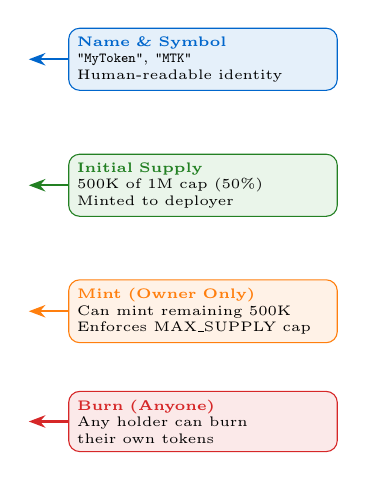
\begin{tikzpicture}[every node/.style={transform shape}]
% Blue callout - name/symbol
\node[draw=mlblue, fill=mlblue!10, rounded corners=4pt, font=\tiny,
      inner sep=3pt, text width=3.2cm, align=left]
      (c1) at (0,4.8) {\textbf{\color{mlblue}Name \& Symbol}\\
      \texttt{"MyToken"}, \texttt{"MTK"}\\
      Human-readable identity};
\draw[-{Stealth[length=6pt]}, mlblue, thick] (c1.west) -- ++(-0.5,0);

% Green callout - initial supply
\node[draw=mlgreen!80!black, fill=mlgreen!10, rounded corners=4pt, font=\tiny,
      inner sep=3pt, text width=3.2cm, align=left]
      (c2) at (0,3.2) {\textbf{\color{mlgreen!80!black}Initial Supply}\\
      500K of 1M cap (50\%)\\
      Minted to deployer};
\draw[-{Stealth[length=6pt]}, mlgreen!80!black, thick] (c2.west) -- ++(-0.5,0);

% Orange callout - mint
\node[draw=mlorange, fill=mlorange!10, rounded corners=4pt, font=\tiny,
      inner sep=3pt, text width=3.2cm, align=left]
      (c3) at (0,1.6) {\textbf{\color{mlorange}Mint (Owner Only)}\\
      Can mint remaining 500K\\
      Enforces MAX\_SUPPLY cap};
\draw[-{Stealth[length=6pt]}, mlorange, thick] (c3.west) -- ++(-0.5,0);

% Red callout - burn
\node[draw=mlred, fill=mlred!10, rounded corners=4pt, font=\tiny,
      inner sep=3pt, text width=3.2cm, align=left]
      (c4) at (0,0.2) {\textbf{\color{mlred}Burn (Anyone)}\\
      Any holder can burn\\
      their own tokens};
\draw[-{Stealth[length=6pt]}, mlred, thick] (c4.west) -- ++(-0.5,0);
\end{tikzpicture}
\end{column}
\end{columns}

\bottomnote{This contract gives you a capped, mintable, burnable ERC-20 token --- 500K minted now, 500K mintable later.}
\end{frame}

%% ============================================================
%% FRAME 5: STEP 2 - DEPLOY ON REMIX (Graphviz-Style DAG)
%% ============================================================
\begin{frame}{Step 2 --- Deploy on Remix}
\vspace{-2mm}
\begin{center}
\adjustbox{max totalheight=6.5cm}{%
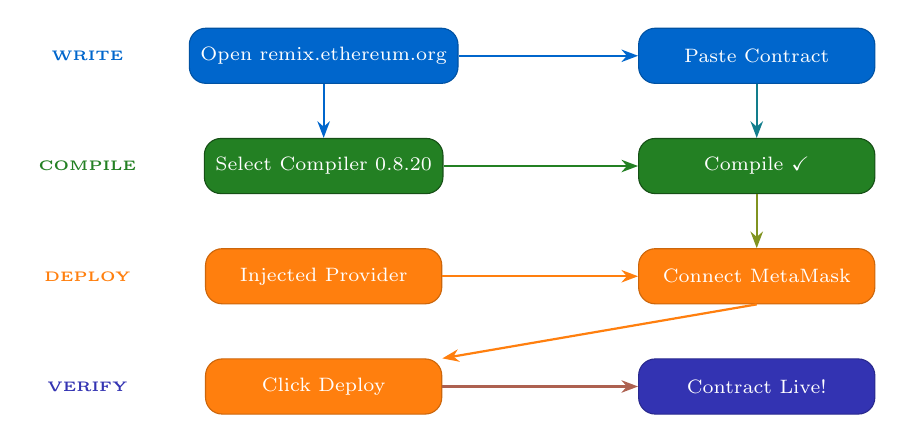
\begin{tikzpicture}[
  node distance=1.0cm and 2.5cm,
  every node/.style={font=\scriptsize, minimum height=0.7cm, minimum width=3.0cm,
                     rounded corners=6pt, align=center, text=white, inner sep=4pt},
  bluebox/.style={fill=mlblue, draw=mlblue!80!black},
  greenbox/.style={fill=mlgreen!80!black, draw=mlgreen!50!black},
  orangebox/.style={fill=mlorange, draw=mlorange!80!black},
  purplebox/.style={fill=mlpurple, draw=mlpurple!80!black},
]

% Row 1
\node[bluebox] (n1) at (0,0) {Open remix.ethereum.org};
\node[bluebox] (n2) at (5.5,0) {Paste Contract};

% Row 2
\node[greenbox] (n3) at (0,-1.4) {Select Compiler 0.8.20};
\node[greenbox] (n4) at (5.5,-1.4) {Compile $\checkmark$};

% Row 3
\node[orangebox] (n5) at (0,-2.8) {Injected Provider};
\node[orangebox] (n6) at (5.5,-2.8) {Connect MetaMask};

% Row 4
\node[orangebox] (n7) at (0,-4.2) {Click Deploy};
\node[purplebox] (n8) at (5.5,-4.2) {Contract Live!};

% Arrows
\draw[-{Stealth[length=6pt]}, mlblue, thick] (n1.east) -- (n2.west);
\draw[-{Stealth[length=6pt]}, mlblue!60!mlgreen, thick] (n2.south) -- (n4.north);
\draw[-{Stealth[length=6pt]}, mlgreen!80!black, thick] (n3.east) -- (n4.west);
\draw[-{Stealth[length=6pt]}, mlgreen!60!mlorange, thick] (n4.south) -- (n6.north);
\draw[-{Stealth[length=6pt]}, mlorange, thick] (n5.east) -- (n6.west);
\draw[-{Stealth[length=6pt]}, mlorange, thick] (n6.south) -- (n7.north east);
\draw[-{Stealth[length=6pt]}, mlorange!60!mlpurple, thick] (n7.east) -- (n8.west);

% Also connect n1 down to n3
\draw[-{Stealth[length=6pt]}, mlblue, thick] (n1.south) -- (n3.north);

% Phase labels
\node[draw=none, fill=none, text=mlblue, font=\tiny\bfseries, minimum width=0cm, minimum height=0cm] at (-3.0,0) {WRITE};
\node[draw=none, fill=none, text=mlgreen!80!black, font=\tiny\bfseries, minimum width=0cm, minimum height=0cm] at (-3.0,-1.4) {COMPILE};
\node[draw=none, fill=none, text=mlorange, font=\tiny\bfseries, minimum width=0cm, minimum height=0cm] at (-3.0,-2.8) {DEPLOY};
\node[draw=none, fill=none, text=mlpurple, font=\tiny\bfseries, minimum width=0cm, minimum height=0cm] at (-3.0,-4.2) {VERIFY};

\end{tikzpicture}
}%
\end{center}

\bottomnote{Remix IDE handles compilation and deployment --- no local tooling required.}
\end{frame}

%% ============================================================
%% FRAME 6: STEP 3 - VERIFY & INTERACT (Comic Strip - 3 panels)
%% ============================================================
\begin{frame}{Step 3 --- Verify \& Interact}
\begin{center}
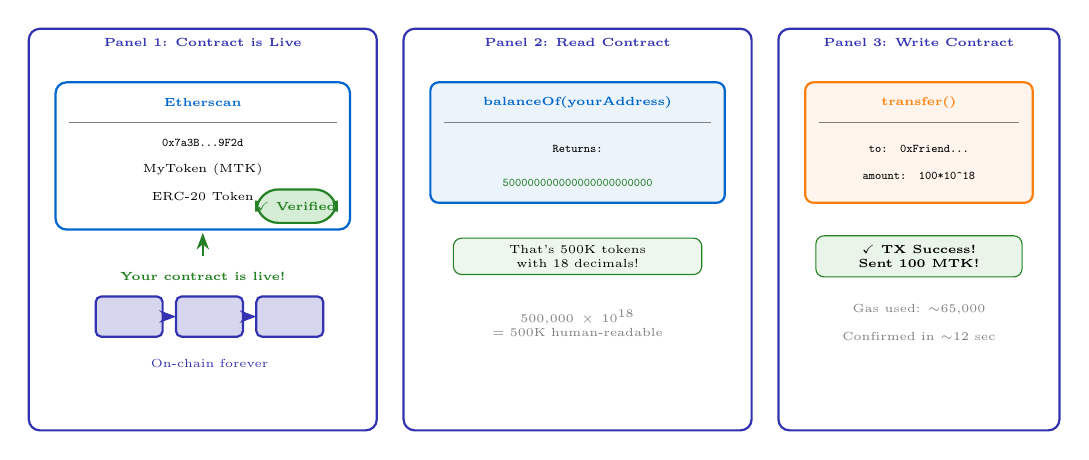
\begin{tikzpicture}[scale=0.85, every node/.style={transform shape}]

% --- Panel 1: Etherscan verification ---
\draw[mlpurple, thick, rounded corners=4pt] (-7.2,-2.8) rectangle (-2.0,3.2);
\node[font=\tiny\bfseries, mlpurple] at (-4.6,3.0) {Panel 1: Contract is Live};

% Etherscan-style box
\draw[mlblue, thick, fill=white, rounded corners=4pt] (-6.8,0.2) rectangle (-2.4,2.4);
\node[font=\tiny\bfseries, mlblue] at (-4.6,2.1) {Etherscan};
\draw[mlgray, thin] (-6.6,1.8) -- (-2.6,1.8);
\node[font=\tiny, align=left] at (-4.6,1.5) {\texttt{0x7a3B...9F2d}};
\node[font=\tiny] at (-4.6,1.1) {MyToken (MTK)};
\node[font=\tiny] at (-4.6,0.7) {ERC-20 Token};

% Green verified badge
\draw[mlgreen!80!black, thick, fill=mlgreen!20, rounded corners=8pt]
     (-3.8,0.3) rectangle (-2.6,0.8);
\node[font=\tiny\bfseries, mlgreen!80!black] at (-3.2,0.55) {$\checkmark$ Verified};

% Arrow pointing to contract
\draw[-{Stealth[length=6pt]}, mlgreen!80!black, thick] (-4.6,-0.2) -- (-4.6,0.15);
\node[font=\tiny\bfseries, mlgreen!80!black] at (-4.6,-0.5) {Your contract is live!};

% Blockchain icon
\draw[mlpurple, thick, fill=mllavender4, rounded corners=2pt] (-6.2,-1.4) rectangle (-5.2,-0.8);
\draw[mlpurple, thick, fill=mllavender4, rounded corners=2pt] (-5.0,-1.4) rectangle (-4.0,-0.8);
\draw[mlpurple, thick, fill=mllavender4, rounded corners=2pt] (-3.8,-1.4) rectangle (-2.8,-0.8);
\draw[-{Stealth[length=6pt]}, mlpurple, thick] (-5.2,-1.1) -- (-5.0,-1.1);
\draw[-{Stealth[length=6pt]}, mlpurple, thick] (-4.0,-1.1) -- (-3.8,-1.1);
\node[font=\tiny, mlpurple] at (-4.5,-1.8) {On-chain forever};

% --- Panel 2: Read Contract ---
\draw[mlpurple, thick, rounded corners=4pt] (-1.6,-2.8) rectangle (3.6,3.2);
\node[font=\tiny\bfseries, mlpurple] at (1.0,3.0) {Panel 2: Read Contract};

% Read panel
\draw[mlblue, thick, fill=mlblue!8, rounded corners=3pt] (-1.2,0.6) rectangle (3.2,2.4);
\node[font=\tiny\bfseries, mlblue] at (1.0,2.1) {balanceOf(yourAddress)};
\draw[mlgray, thin] (-1.0,1.8) -- (3.0,1.8);
\node[font=\tiny, align=center] at (1.0,1.4) {\texttt{Returns:}};
\node[font=\tiny\bfseries, mlgreen!80!black, text width=3.5cm, align=center] at (1.0,0.9) {\texttt{500000000000000000000000}};

% Annotation
\node[draw=mlgreen!80!black, fill=mlgreen!8, rounded corners=3pt, font=\tiny,
      inner sep=3pt, text width=3.5cm, align=center]
      at (1.0,-0.2) {That's 500K tokens\\with 18 decimals!};

% Decimal explanation
\node[font=\tiny, mlgray, text width=3.5cm, align=center]
      at (1.0,-1.2) {$500{,}000 \times 10^{18}$\\= 500K human-readable};

% --- Panel 3: Write Contract ---
\draw[mlpurple, thick, rounded corners=4pt] (4.0,-2.8) rectangle (8.2,3.2);
\node[font=\tiny\bfseries, mlpurple] at (6.1,3.0) {Panel 3: Write Contract};

% Write panel
\draw[mlorange, thick, fill=mlorange!8, rounded corners=3pt] (4.4,0.6) rectangle (7.8,2.4);
\node[font=\tiny\bfseries, mlorange] at (6.1,2.1) {transfer()};
\draw[mlgray, thin] (4.6,1.8) -- (7.6,1.8);
\node[font=\tiny, align=left] at (6.1,1.4) {\texttt{to: 0xFriend...}};
\node[font=\tiny, align=left] at (6.1,1.0) {\texttt{amount: 100*10\^{}18}};

% Success message
\node[draw=mlgreen!80!black, fill=mlgreen!10, rounded corners=3pt, font=\tiny\bfseries,
      inner sep=4pt, text width=2.8cm, align=center]
      at (6.1,-0.2) {$\checkmark$ TX Success!\\Sent 100 MTK!};

% Gas info
\node[font=\tiny, mlgray] at (6.1,-1.0) {Gas used: $\sim$65,000};
\node[font=\tiny, mlgray] at (6.1,-1.4) {Confirmed in $\sim$12 sec};

\end{tikzpicture}
\end{center}

\bottomnote{Once deployed, anyone can read your contract and interact with your token.}
\end{frame}

%% ============================================================
%% FRAME 7: STEP 4 - ADD TO METAMASK & SHARE (Radial Graph)
%% ============================================================
\begin{frame}{Step 4 --- Add to MetaMask \& Share}
\vspace{-2mm}
\begin{center}
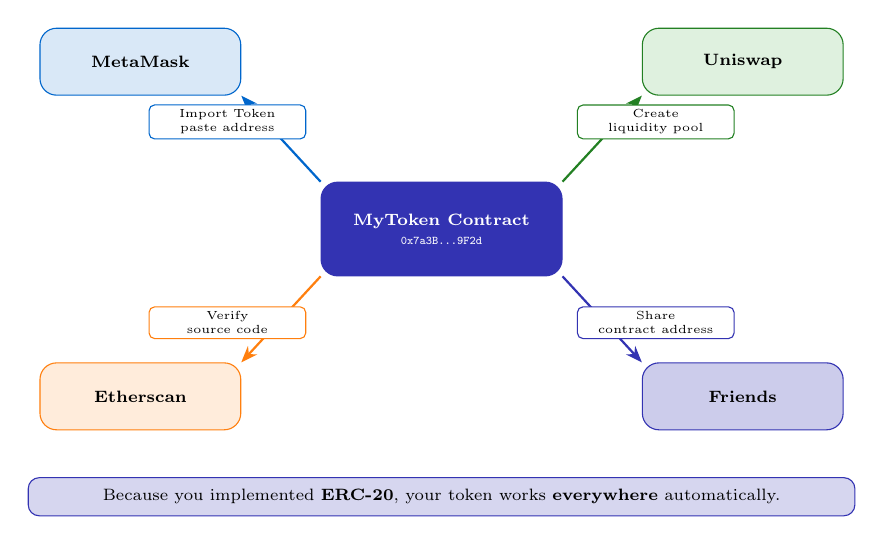
\begin{tikzpicture}[scale=0.85, every node/.style={transform shape}]

% Central node
\node[draw=mlpurple, fill=mlpurple, text=white, rounded corners=6pt,
      minimum width=3.6cm, minimum height=1.4cm, font=\scriptsize\bfseries,
      align=center] (center) at (0,0.5) {MyToken Contract\\{\tiny\texttt{0x7a3B...9F2d}}};

% MetaMask (top-left, blue)
\node[draw=mlblue, fill=mlblue!15, rounded corners=6pt,
      minimum width=3.0cm, minimum height=1.0cm, font=\scriptsize\bfseries,
      align=center] (mm) at (-4.5,3.0) {MetaMask};

% Uniswap (top-right, green)
\node[draw=mlgreen!80!black, fill=mlgreen!15, rounded corners=6pt,
      minimum width=3.0cm, minimum height=1.0cm, font=\scriptsize\bfseries,
      align=center] (uni) at (4.5,3.0) {Uniswap};

% Etherscan (bottom-left, orange)
\node[draw=mlorange, fill=mlorange!15, rounded corners=6pt,
      minimum width=3.0cm, minimum height=1.0cm, font=\scriptsize\bfseries,
      align=center] (eth) at (-4.5,-2.0) {Etherscan};

% Friends (bottom-right, purple)
\node[draw=mlpurple, fill=mllavender3, rounded corners=6pt,
      minimum width=3.0cm, minimum height=1.0cm, font=\scriptsize\bfseries,
      align=center] (fri) at (4.5,-2.0) {Friends};

% Arrows with labels
\draw[-{Stealth[length=6pt]}, mlblue, thick] (center.north west) -- (mm.south east);
\node[draw=mlblue, fill=white, rounded corners=2pt, font=\tiny, inner sep=2pt,
      text width=2.2cm, align=center] at (-3.2,2.1) {Import Token\\paste address};

\draw[-{Stealth[length=6pt]}, mlgreen!80!black, thick] (center.north east) -- (uni.south west);
\node[draw=mlgreen!80!black, fill=white, rounded corners=2pt, font=\tiny, inner sep=2pt,
      text width=2.2cm, align=center] at (3.2,2.1) {Create\\liquidity pool};

\draw[-{Stealth[length=6pt]}, mlorange, thick] (center.south west) -- (eth.north east);
\node[draw=mlorange, fill=white, rounded corners=2pt, font=\tiny, inner sep=2pt,
      text width=2.2cm, align=center] at (-3.2,-0.9) {Verify\\source code};

\draw[-{Stealth[length=6pt]}, mlpurple, thick] (center.south east) -- (fri.north west);
\node[draw=mlpurple, fill=white, rounded corners=2pt, font=\tiny, inner sep=2pt,
      text width=2.2cm, align=center] at (3.2,-0.9) {Share\\contract address};

% Key insight box at bottom
\node[draw=mlpurple, fill=mllavender4, rounded corners=4pt, font=\scriptsize,
      inner sep=5pt, text width=12cm, align=center] at (0,-3.5)
     {Because you implemented \textbf{ERC-20}, your token works \textbf{everywhere} automatically.};

\end{tikzpicture}
\end{center}

\bottomnote{ERC-20 compliance means instant compatibility with the entire Ethereum ecosystem.}
\end{frame}

%% ============================================================
%% FRAME 8: PART B SECTION DIVIDER
%% ============================================================
\begin{frame}{}
\vfill
\begin{beamercolorbox}[sep=12pt,center,rounded=true,shadow=true]{palette quaternary}
{\Large\bfseries Part 2: Deep Dive --- The Technical Details}\\[6pt]
{\normalsize Formal explanations behind five key concepts from the visual introduction}
\end{beamercolorbox}
\vfill
\end{frame}

%% ============================================================
%% FRAME 9: HOW TOKENS WORK - THE BALANCE MAPPING [fragile]
%% ============================================================
\begin{frame}[fragile]{How Tokens Actually Work --- The Balance Mapping}
\vspace{-3mm}
\begin{center}
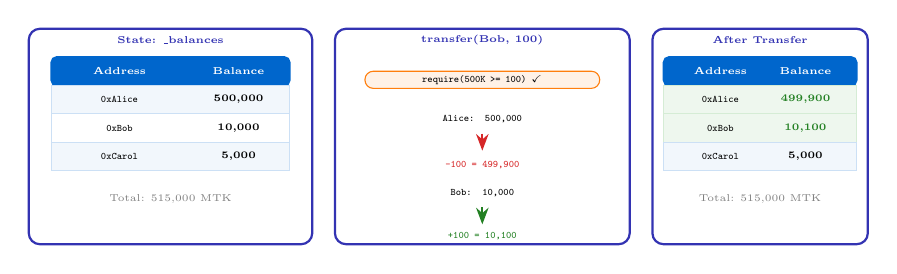
\begin{tikzpicture}[scale=0.72, every node/.style={transform shape}]

% --- Panel 1: Initial mapping ---
\draw[mlpurple, thick, rounded corners=4pt] (-7.2,-0.6) rectangle (-2.2,3.2);
\node[font=\tiny\bfseries, mlpurple] at (-4.7,3.0) {State: \_balances};

% Table header
\draw[mlblue, thick, fill=mlblue, rounded corners=2pt] (-6.8,2.2) rectangle (-2.6,2.7);
\node[font=\tiny\bfseries, white] at (-5.6,2.45) {Address};
\node[font=\tiny\bfseries, white] at (-3.5,2.45) {Balance};

% Table rows
\draw[mlblue!20, fill=mlblue!5] (-6.8,1.7) rectangle (-2.6,2.2);
\node[font=\tiny] at (-5.6,1.95) {\texttt{0xAlice}};
\node[font=\tiny\bfseries] at (-3.5,1.95) {500,000};

\draw[mlblue!20, fill=white] (-6.8,1.2) rectangle (-2.6,1.7);
\node[font=\tiny] at (-5.6,1.45) {\texttt{0xBob}};
\node[font=\tiny\bfseries] at (-3.5,1.45) {10,000};

\draw[mlblue!20, fill=mlblue!5] (-6.8,0.7) rectangle (-2.6,1.2);
\node[font=\tiny] at (-5.6,0.95) {\texttt{0xCarol}};
\node[font=\tiny\bfseries] at (-3.5,0.95) {5,000};

\node[font=\tiny, mlgray] at (-4.7,0.2) {Total: 515,000 MTK};

% --- Panel 2: Transfer operation ---
\draw[mlpurple, thick, rounded corners=4pt] (-1.8,-0.6) rectangle (3.4,3.2);
\node[font=\tiny\bfseries, mlpurple] at (0.8,3.0) {transfer(Bob, 100)};

% Require check
\node[draw=mlorange, fill=mlorange!10, rounded corners=3pt, font=\tiny,
      inner sep=2pt, text width=4.0cm, align=center]
      at (0.8,2.3) {\texttt{require(500K >= 100)} $\checkmark$};

% Alice balance decrease
\node[font=\tiny, align=center] at (0.8,1.6) {\texttt{Alice: 500,000}};
\draw[-{Stealth[length=6pt]}, mlred, thick] (0.8,1.35) -- (0.8,1.05);
\node[font=\tiny\bfseries, mlred] at (0.8,0.8) {\texttt{-100 = 499,900}};

% Bob balance increase
\node[font=\tiny, align=center] at (0.8,0.3) {\texttt{Bob: 10,000}};
\draw[-{Stealth[length=6pt]}, mlgreen!80!black, thick] (0.8,0.05) -- (0.8,-0.25);
\node[font=\tiny\bfseries, mlgreen!80!black] at (0.8,-0.45) {\texttt{+100 = 10,100}};

% --- Panel 3: Updated mapping ---
\draw[mlpurple, thick, rounded corners=4pt] (3.8,-0.6) rectangle (7.6,3.2);
\node[font=\tiny\bfseries, mlpurple] at (5.7,3.0) {After Transfer};

% Table header
\draw[mlblue, thick, fill=mlblue, rounded corners=2pt] (4.0,2.2) rectangle (7.4,2.7);
\node[font=\tiny\bfseries, white] at (5.0,2.45) {Address};
\node[font=\tiny\bfseries, white] at (6.5,2.45) {Balance};

% Updated rows - changed values highlighted
\draw[mlgreen!20, fill=mlgreen!8] (4.0,1.7) rectangle (7.4,2.2);
\node[font=\tiny] at (5.0,1.95) {\texttt{0xAlice}};
\node[font=\tiny\bfseries, mlgreen!80!black] at (6.5,1.95) {499,900};

\draw[mlgreen!20, fill=mlgreen!8] (4.0,1.2) rectangle (7.4,1.7);
\node[font=\tiny] at (5.0,1.45) {\texttt{0xBob}};
\node[font=\tiny\bfseries, mlgreen!80!black] at (6.5,1.45) {10,100};

\draw[mlblue!20, fill=mlblue!5] (4.0,0.7) rectangle (7.4,1.2);
\node[font=\tiny] at (5.0,0.95) {\texttt{0xCarol}};
\node[font=\tiny\bfseries] at (6.5,0.95) {5,000};

\node[font=\tiny, mlgray] at (5.7,0.2) {Total: 515,000 MTK};

\end{tikzpicture}
\end{center}
\vspace{-2mm}
\begin{lstlisting}[basicstyle=\ttfamily\tiny,xleftmargin=0pt,xrightmargin=0pt,linewidth=\linewidth]
mapping(address => uint256) private _balances;
function transfer(address to, uint256 amount) public returns (bool) {
    require(_balances[msg.sender] >= amount, "Insufficient");
    _balances[msg.sender] -= amount;
    _balances[to] += amount;
    emit Transfer(msg.sender, to, amount);
    return true;
}
\end{lstlisting}

\bottomnote{A token is just a mapping from addresses to balances --- the smart contract is the ledger.}
\end{frame}

%% ============================================================
%% FRAME 10: THE ERC-20 INTERFACE (Graphviz Dependency Graph)
%% ============================================================
\begin{frame}{The ERC-20 Interface --- All 6 Functions}
\vspace{-2mm}
\begin{center}
\adjustbox{max totalheight=6.5cm}{%
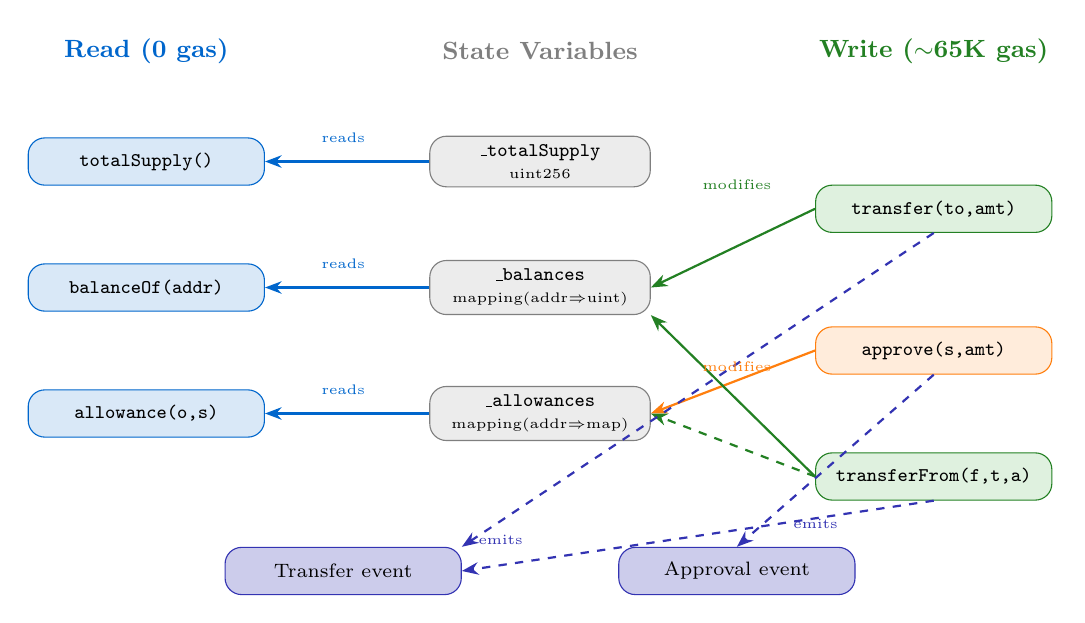
\begin{tikzpicture}[
  every node/.style={font=\scriptsize, rounded corners=6pt, align=center,
                     minimum height=0.6cm, inner sep=3pt},
]

% === Column headers ===
\node[draw=none, fill=none, font=\small\bfseries, mlblue] at (-5.0,5.2) {Read (0 gas)};
\node[draw=none, fill=none, font=\small\bfseries, mlgray] at (0,5.2) {State Variables};
\node[draw=none, fill=none, font=\small\bfseries, mlgreen!80!black] at (5.0,5.2) {Write ($\sim$65K gas)};

% === State variables (center) ===
\node[draw=mlgray, fill=mlgray!15, minimum width=2.8cm]
      (ts) at (0,3.8) {\texttt{\_totalSupply}\\{\tiny uint256}};
\node[draw=mlgray, fill=mlgray!15, minimum width=2.8cm]
      (bal) at (0,2.2) {\texttt{\_balances}\\{\tiny mapping(addr$\Rightarrow$uint)}};
\node[draw=mlgray, fill=mlgray!15, minimum width=2.8cm]
      (alw) at (0,0.6) {\texttt{\_allowances}\\{\tiny mapping(addr$\Rightarrow$map)}};

% === Read functions (left, blue) ===
\node[draw=mlblue, fill=mlblue!15, minimum width=3.0cm]
      (f1) at (-5.0,3.8) {\texttt{totalSupply()}};
\node[draw=mlblue, fill=mlblue!15, minimum width=3.0cm]
      (f2) at (-5.0,2.2) {\texttt{balanceOf(addr)}};
\node[draw=mlblue, fill=mlblue!15, minimum width=3.0cm]
      (f3) at (-5.0,0.6) {\texttt{allowance(o,s)}};

% === Write functions (right, green/orange) ===
\node[draw=mlgreen!80!black, fill=mlgreen!15, minimum width=3.0cm]
      (f4) at (5.0,3.2) {\texttt{transfer(to,amt)}};
\node[draw=mlorange, fill=mlorange!15, minimum width=3.0cm]
      (f5) at (5.0,1.4) {\texttt{approve(s,amt)}};
\node[draw=mlgreen!80!black, fill=mlgreen!15, minimum width=3.0cm]
      (f6) at (5.0,-0.2) {\texttt{transferFrom(f,t,a)}};

% === Events (bottom row, purple) ===
\node[draw=mlpurple, fill=mllavender3, minimum width=3.0cm]
      (e1) at (-2.5,-1.4) {Transfer event};
\node[draw=mlpurple, fill=mllavender3, minimum width=3.0cm]
      (e2) at (2.5,-1.4) {Approval event};

% === Arrows: reads ===
\draw[-{Stealth[length=6pt]}, mlblue, thick] (ts.west) -- (f1.east);
\draw[-{Stealth[length=6pt]}, mlblue, thick] (bal.west) -- (f2.east);
\draw[-{Stealth[length=6pt]}, mlblue, thick] (alw.west) -- (f3.east);

% === Arrows: writes ===
\draw[-{Stealth[length=6pt]}, mlgreen!80!black, thick] (f4.west) -- (bal.east);
\draw[-{Stealth[length=6pt]}, mlorange, thick] (f5.west) -- (alw.east);
\draw[-{Stealth[length=6pt]}, mlgreen!80!black, thick] (f6.west) -- (bal.south east);
\draw[-{Stealth[length=6pt]}, mlgreen!80!black, thick, dashed] (f6.west) -- (alw.east);

% === Arrows: events ===
\draw[-{Stealth[length=6pt]}, mlpurple, thick, dashed] (f4.south) -- (e1.north east);
\draw[-{Stealth[length=6pt]}, mlpurple, thick, dashed] (f5.south) -- (e2.north);
\draw[-{Stealth[length=6pt]}, mlpurple, thick, dashed] (f6.south) -- (e1.east);

% Labels on arrows
\node[draw=none, fill=none, font=\tiny, mlblue] at (-2.5,4.1) {reads};
\node[draw=none, fill=none, font=\tiny, mlblue] at (-2.5,2.5) {reads};
\node[draw=none, fill=none, font=\tiny, mlblue] at (-2.5,0.9) {reads};
\node[draw=none, fill=none, font=\tiny, mlgreen!80!black] at (2.5,3.5) {modifies};
\node[draw=none, fill=none, font=\tiny, mlorange] at (2.5,1.2) {modifies};
\node[draw=none, fill=none, font=\tiny, mlpurple] at (-0.5,-1.0) {emits};
\node[draw=none, fill=none, font=\tiny, mlpurple] at (3.5,-0.8) {emits};

\end{tikzpicture}
}%
\end{center}

\bottomnote{Read functions cost zero gas; write functions require a transaction and pay gas.}
\end{frame}

%% ============================================================
%% FRAME 11: TRANSFER VS APPROVE - THE FULL MECHANISM [fragile]
%% ============================================================
\begin{frame}[fragile]{Transfer vs Approve --- The Full Mechanism}
\vspace{-3mm}
\begin{center}
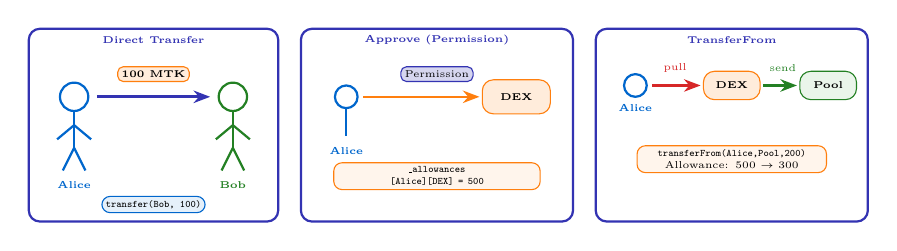
\begin{tikzpicture}[scale=0.72, every node/.style={transform shape}]

% --- Panel 1: Direct transfer ---
\draw[mlpurple, thick, rounded corners=4pt] (-7.2,-0.4) rectangle (-2.8,3.0);
\node[font=\tiny\bfseries, mlpurple] at (-5.0,2.8) {Direct Transfer};

% Alice stick figure (small)
\draw[mlblue, thick] (-6.4,1.8) circle (0.25);
\draw[mlblue, thick] (-6.4,1.55) -- (-6.4,0.9);
\draw[mlblue, thick] (-6.4,1.3) -- (-6.7,1.05);
\draw[mlblue, thick] (-6.4,1.3) -- (-6.1,1.05);
\draw[mlblue, thick] (-6.4,0.9) -- (-6.6,0.5);
\draw[mlblue, thick] (-6.4,0.9) -- (-6.2,0.5);
\node[font=\tiny\bfseries, mlblue] at (-6.4,0.25) {Alice};

% Bob stick figure
\draw[mlgreen!80!black, thick] (-3.6,1.8) circle (0.25);
\draw[mlgreen!80!black, thick] (-3.6,1.55) -- (-3.6,0.9);
\draw[mlgreen!80!black, thick] (-3.6,1.3) -- (-3.9,1.05);
\draw[mlgreen!80!black, thick] (-3.6,1.3) -- (-3.3,1.05);
\draw[mlgreen!80!black, thick] (-3.6,0.9) -- (-3.8,0.5);
\draw[mlgreen!80!black, thick] (-3.6,0.9) -- (-3.4,0.5);
\node[font=\tiny\bfseries, mlgreen!80!black] at (-3.6,0.25) {Bob};

% Arrow
\draw[-{Stealth[length=6pt]}, mlpurple, very thick] (-6.0,1.8) -- (-4.0,1.8);
\node[draw=mlorange, fill=mlorange!15, rounded corners=2pt, font=\tiny\bfseries,
      inner sep=2pt] at (-5.0,2.2) {100 MTK};

% Function label
\node[draw=mlblue, fill=mlblue!10, rounded corners=3pt, font=\tiny\bfseries,
      inner sep=2pt] at (-5.0,-0.1) {\texttt{transfer(Bob, 100)}};

% --- Panel 2: Approve step ---
\draw[mlpurple, thick, rounded corners=4pt] (-2.4,-0.4) rectangle (2.4,3.0);
\node[font=\tiny\bfseries, mlpurple] at (0,2.8) {Approve (Permission)};

% Alice (small)
\draw[mlblue, thick] (-1.6,1.8) circle (0.2);
\draw[mlblue, thick] (-1.6,1.6) -- (-1.6,1.1);
\node[font=\tiny\bfseries, mlblue] at (-1.6,0.85) {Alice};

% DEX box
\node[draw=mlorange, fill=mlorange!15, rounded corners=4pt,
      minimum width=1.2cm, minimum height=0.6cm, font=\tiny\bfseries]
      (dex) at (1.4,1.8) {DEX};

% Permission arrow
\draw[-{Stealth[length=6pt]}, mlorange, thick] (-1.3,1.8) -- (0.75,1.8);
\node[draw=mlpurple, fill=mllavender4, rounded corners=2pt, font=\tiny,
      inner sep=2pt] at (0,2.2) {Permission};

% Allowance mapping visual
\node[draw=mlorange, fill=mlorange!8, rounded corners=3pt, font=\tiny,
      inner sep=2pt, text width=3.5cm, align=center]
      at (0,0.4) {\texttt{\_allowances}\\
      \texttt{[Alice][DEX] = 500}};

% --- Panel 3: TransferFrom ---
\draw[mlpurple, thick, rounded corners=4pt] (2.8,-0.4) rectangle (7.6,3.0);
\node[font=\tiny\bfseries, mlpurple] at (5.2,2.8) {TransferFrom};

% Alice (source, small)
\draw[mlblue, thick] (3.5,2.0) circle (0.2);
\node[font=\tiny\bfseries, mlblue] at (3.5,1.6) {Alice};

% DEX (orchestrator)
\node[draw=mlorange, fill=mlorange!15, rounded corners=4pt,
      minimum width=1.0cm, minimum height=0.5cm, font=\tiny\bfseries]
      (dex2) at (5.2,2.0) {DEX};

% Pool (destination)
\node[draw=mlgreen!80!black, fill=mlgreen!10, rounded corners=4pt,
      minimum width=1.0cm, minimum height=0.5cm, font=\tiny\bfseries]
      (pool) at (6.9,2.0) {Pool};

% Arrows
\draw[-{Stealth[length=6pt]}, mlred, thick] (3.8,2.0) -- (4.65,2.0);
\node[font=\tiny, mlred] at (4.2,2.3) {pull};
\draw[-{Stealth[length=6pt]}, mlgreen!80!black, thick] (5.75,2.0) -- (6.35,2.0);
\node[font=\tiny, mlgreen!80!black] at (6.1,2.3) {send};

% Allowance update
\node[draw=mlorange, fill=mlorange!8, rounded corners=3pt, font=\tiny,
      inner sep=2pt, text width=3.2cm, align=center]
      at (5.2,0.7) {\texttt{transferFrom(Alice,Pool,200)}\\
      Allowance: 500 $\rightarrow$ 300};

\end{tikzpicture}
\end{center}
\vspace{-1mm}
% Red warning box
\begin{center}
\colorbox{mlred!10}{\parbox{0.9\linewidth}{\centering\tiny\bfseries\color{mlred}
Race condition warning: set allowance to 0 first, then set to new value}}
\end{center}
\vspace{-2mm}
\begin{lstlisting}[basicstyle=\ttfamily\tiny,xleftmargin=0pt,xrightmargin=0pt,linewidth=\linewidth]
mapping(address => mapping(address => uint256))
    private _allowances;
function approve(address spender, uint256 amount)
    public returns (bool) {
    _allowances[msg.sender][spender] = amount;
    emit Approval(msg.sender, spender, amount);
    return true;
}
\end{lstlisting}

\bottomnote{approve()+transferFrom() is the delegation pattern that powers all of DeFi.}
\end{frame}

%% ============================================================
%% FRAME 12: TOKEN SUPPLY MODELS - THE MATHEMATICS [fragile]
%% ============================================================
\begin{frame}[fragile]{Token Supply Models --- The Mathematics}
\vspace{-3mm}
\begin{columns}[T]

% === Column 1: Fixed Supply ===
\begin{column}{0.32\linewidth}
\begin{center}
{\small\bfseries\color{mlblue} Fixed Supply}\\[2mm]
\adjustbox{max width=\linewidth}{%
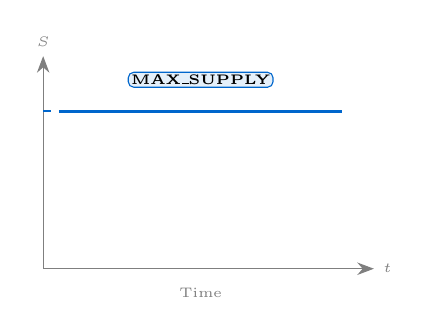
\begin{tikzpicture}
\draw[mlgray, thin, -{Stealth[length=6pt]}] (0,0) -- (4.2,0) node[right, font=\tiny]{$t$};
\draw[mlgray, thin, -{Stealth[length=6pt]}] (0,0) -- (0,2.7) node[above, font=\tiny]{$S$};
\draw[mlblue, very thick] (0.2,2.0) -- (3.8,2.0);
\draw[mlblue, thick, dashed] (0,2.0) -- (0.2,2.0);
\node[draw=mlblue, fill=mlblue!10, rounded corners=2pt, font=\tiny\bfseries,
      inner sep=1pt] at (2.0,2.4) {MAX\_SUPPLY};
\node[font=\tiny, mlgray] at (2.0,-0.3) {Time};
\end{tikzpicture}
}%
\\[2mm]
$S(t) = S_0, \quad \forall\, t \geq 0$
\\[2mm]
\adjustbox{max width=\linewidth}{%
\begin{lstlisting}[basicstyle=\ttfamily\tiny,numbers=none,frame=none,backgroundcolor=\color{mlblue!8},xleftmargin=0pt,xrightmargin=0pt]
uint256 public constant
  MAX_SUPPLY = 1_000_000 * 10**18;
\end{lstlisting}}%
\end{center}
\end{column}

% === Column 2: Inflationary ===
\begin{column}{0.32\linewidth}
\begin{center}
{\small\bfseries\color{mlgreen!80!black} Inflationary}\\[2mm]
\adjustbox{max width=\linewidth}{%
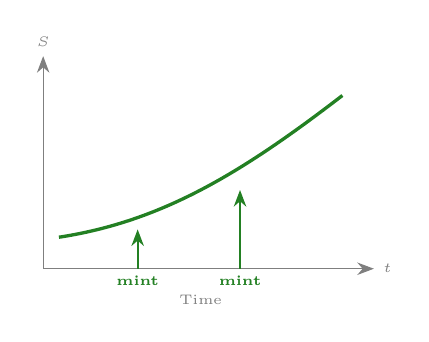
\begin{tikzpicture}
\draw[mlgray, thin, -{Stealth[length=6pt]}] (0,0) -- (4.2,0) node[right, font=\tiny]{$t$};
\draw[mlgray, thin, -{Stealth[length=6pt]}] (0,0) -- (0,2.7) node[above, font=\tiny]{$S$};
\draw[mlgreen!80!black, very thick] (0.2,0.4) .. controls (1.5,0.6) and (2.5,1.2) .. (3.8,2.2);
\draw[-{Stealth[length=6pt]}, mlgreen!80!black, thick] (1.2,0) -- (1.2,0.5);
\node[font=\tiny\bfseries, mlgreen!80!black] at (1.2,-0.15) {mint};
\draw[-{Stealth[length=6pt]}, mlgreen!80!black, thick] (2.5,0) -- (2.5,1.0);
\node[font=\tiny\bfseries, mlgreen!80!black] at (2.5,-0.15) {mint};
\node[font=\tiny, mlgray] at (2.0,-0.4) {Time};
\end{tikzpicture}
}%
\\[2mm]
$S_n = S_0 + \displaystyle\sum_{i=1}^{n} m_i$
\\[2mm]
\adjustbox{max width=\linewidth}{%
\begin{lstlisting}[basicstyle=\ttfamily\tiny,numbers=none,frame=none,backgroundcolor=\color{mlgreen!8},xleftmargin=0pt,xrightmargin=0pt]
function mint(address to, uint256 a)
  onlyOwner { _mint(to, a); }
\end{lstlisting}}%
\end{center}
\end{column}

% === Column 3: Deflationary ===
\begin{column}{0.32\linewidth}
\begin{center}
{\small\bfseries\color{mlred} Deflationary}\\[2mm]
\adjustbox{max width=\linewidth}{%
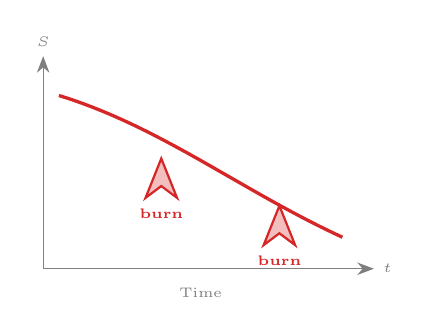
\begin{tikzpicture}
\draw[mlgray, thin, -{Stealth[length=6pt]}] (0,0) -- (4.2,0) node[right, font=\tiny]{$t$};
\draw[mlgray, thin, -{Stealth[length=6pt]}] (0,0) -- (0,2.7) node[above, font=\tiny]{$S$};
\draw[mlred, very thick] (0.2,2.2) .. controls (1.5,1.8) and (2.5,1.0) .. (3.8,0.4);
% Burn flames
\draw[mlred, thick, fill=mlred!30] (1.5,1.4) -- (1.3,0.9) -- (1.5,1.05) -- (1.7,0.9) -- cycle;
\node[font=\tiny\bfseries, mlred] at (1.5,0.7) {burn};
\draw[mlred, thick, fill=mlred!30] (3.0,0.8) -- (2.8,0.3) -- (3.0,0.45) -- (3.2,0.3) -- cycle;
\node[font=\tiny\bfseries, mlred] at (3.0,0.1) {burn};
\node[font=\tiny, mlgray] at (2.0,-0.3) {Time};
\end{tikzpicture}
}%
\\[2mm]
$S_n = S_0 - \displaystyle\sum_{i=1}^{n} b_i$
\\[2mm]
\adjustbox{max width=\linewidth}{%
\begin{lstlisting}[basicstyle=\ttfamily\tiny,numbers=none,frame=none,backgroundcolor=\color{mlred!8},xleftmargin=0pt,xrightmargin=0pt]
function burn(uint256 amt) public {
    _burn(msg.sender, amt); }
\end{lstlisting}}%
\end{center}
\end{column}

\end{columns}

\bottomnote{Tokenomics = mathematical models governing supply evolution via mint and burn events.}
\end{frame}

%% ============================================================
%% FRAME 13: SECURITY - WHY OPENZEPPELIN? (Attack/Defense Tree)
%% ============================================================
\begin{frame}{Security --- Why OpenZeppelin?}
\vspace{-2mm}
\begin{center}
\adjustbox{max width=\textwidth,max totalheight=6.5cm}{%
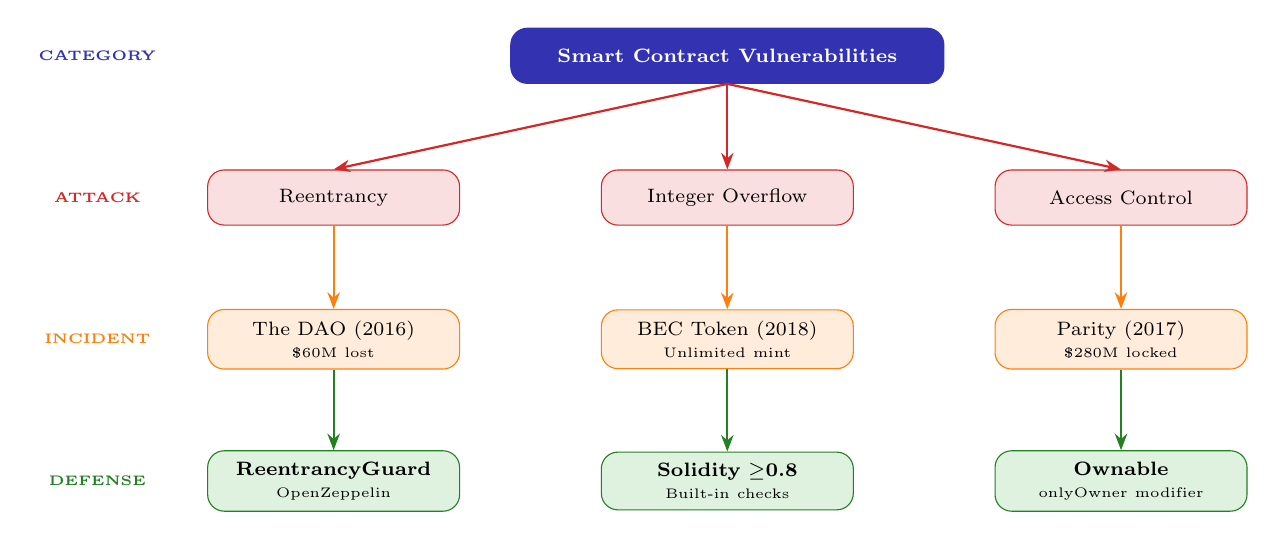
\begin{tikzpicture}[
  every node/.style={font=\scriptsize, rounded corners=6pt, align=center,
                     minimum height=0.7cm, inner sep=4pt},
]

% Level 0: Root
\node[draw=mlpurple, fill=mlpurple, text=white, minimum width=5.5cm, font=\scriptsize\bfseries]
      (root) at (0,0) {Smart Contract Vulnerabilities};

% Level 1: Attack types (red)
\node[draw=mlred, fill=mlred!15, minimum width=3.2cm]
      (a1) at (-5.0,-1.8) {Reentrancy};
\node[draw=mlred, fill=mlred!15, minimum width=3.2cm]
      (a2) at (0,-1.8) {Integer Overflow};
\node[draw=mlred, fill=mlred!15, minimum width=3.2cm]
      (a3) at (5.0,-1.8) {Access Control};

% Level 2: Real incidents (orange)
\node[draw=mlorange, fill=mlorange!15, minimum width=3.2cm, text width=2.8cm]
      (i1) at (-5.0,-3.6) {The DAO (2016)\\{\tiny \$60M lost}};
\node[draw=mlorange, fill=mlorange!15, minimum width=3.2cm, text width=2.8cm]
      (i2) at (0,-3.6) {BEC Token (2018)\\{\tiny Unlimited mint}};
\node[draw=mlorange, fill=mlorange!15, minimum width=3.2cm, text width=2.8cm]
      (i3) at (5.0,-3.6) {Parity (2017)\\{\tiny \$280M locked}};

% Level 3: OpenZeppelin defenses (green)
\node[draw=mlgreen!80!black, fill=mlgreen!15, minimum width=3.2cm, text width=2.8cm]
      (d1) at (-5.0,-5.4) {\textbf{ReentrancyGuard}\\{\tiny OpenZeppelin}};
\node[draw=mlgreen!80!black, fill=mlgreen!15, minimum width=3.2cm, text width=2.8cm]
      (d2) at (0,-5.4) {\textbf{Solidity $\geq$0.8}\\{\tiny Built-in checks}};
\node[draw=mlgreen!80!black, fill=mlgreen!15, minimum width=3.2cm, text width=2.8cm]
      (d3) at (5.0,-5.4) {\textbf{Ownable}\\{\tiny onlyOwner modifier}};

% All arrows downward
\draw[-{Stealth[length=6pt]}, mlred, thick] (root.south) -- (a1.north);
\draw[-{Stealth[length=6pt]}, mlred, thick] (root.south) -- (a2.north);
\draw[-{Stealth[length=6pt]}, mlred, thick] (root.south) -- (a3.north);

\draw[-{Stealth[length=6pt]}, mlorange, thick] (a1.south) -- (i1.north);
\draw[-{Stealth[length=6pt]}, mlorange, thick] (a2.south) -- (i2.north);
\draw[-{Stealth[length=6pt]}, mlorange, thick] (a3.south) -- (i3.north);

\draw[-{Stealth[length=6pt]}, mlgreen!80!black, thick] (i1.south) -- (d1.north);
\draw[-{Stealth[length=6pt]}, mlgreen!80!black, thick] (i2.south) -- (d2.north);
\draw[-{Stealth[length=6pt]}, mlgreen!80!black, thick] (i3.south) -- (d3.north);

% Level labels on the side
\node[draw=none, fill=none, font=\tiny\bfseries, mlpurple, minimum height=0cm, minimum width=0cm]
      at (-8.0,0) {CATEGORY};
\node[draw=none, fill=none, font=\tiny\bfseries, mlred, minimum height=0cm, minimum width=0cm]
      at (-8.0,-1.8) {ATTACK};
\node[draw=none, fill=none, font=\tiny\bfseries, mlorange, minimum height=0cm, minimum width=0cm]
      at (-8.0,-3.6) {INCIDENT};
\node[draw=none, fill=none, font=\tiny\bfseries, mlgreen!80!black, minimum height=0cm, minimum width=0cm]
      at (-8.0,-5.4) {DEFENSE};

\end{tikzpicture}
}%
\end{center}

\bottomnote{Smart contract bugs are permanent and immutable --- use audited libraries, always.}
\end{frame}

%% ============================================================
%% FRAME 14: KEY TERMS FOR BEGINNERS
%% ============================================================
\begin{frame}{Key Terms for Beginners}
\vspace{-2mm}
\begin{columns}[T]
\begin{column}{0.48\linewidth}
\renewcommand{\arraystretch}{1.15}
{\scriptsize
\begin{tabular}{@{}p{1.8cm}p{4.8cm}@{}}
\toprule
\textbf{\color{mlpurple}Term} & \textbf{\color{mlpurple}Definition} \\
\midrule
\textbf{Blockchain} & A shared, tamper-proof digital ledger that records every transaction across a network of computers. \\
\textbf{Ethereum} & A blockchain platform that supports smart contracts and is home to most ERC-20 tokens. \\
\textbf{Smart Contract} & A self-executing program on the blockchain that enforces rules automatically, without intermediaries. \\
\textbf{Token} & A digital asset created by a smart contract on an existing blockchain (unlike a coin, which has its own chain). \\
\textbf{ERC-20} & The standard interface (6 functions + 2 events) that all fungible tokens on Ethereum must implement. \\
\textbf{Fungible} & Interchangeable; one token equals any other of the same type, like dollar bills. \\
\textbf{Solidity} & The programming language used to write smart contracts on Ethereum. \\
\textbf{Remix IDE} & A free, browser-based tool for writing, compiling, and deploying Solidity smart contracts. \\
\textbf{Gas} & A fee (paid in ETH) for executing operations on Ethereum; every transaction costs gas. \\
\textbf{Wallet} & Software (e.g., MetaMask) that stores your private keys and lets you interact with the blockchain. \\
\bottomrule
\end{tabular}
}
\end{column}
\begin{column}{0.48\linewidth}
\renewcommand{\arraystretch}{1.15}
{\scriptsize
\begin{tabular}{@{}p{1.8cm}p{4.8cm}@{}}
\toprule
\textbf{\color{mlpurple}Term} & \textbf{\color{mlpurple}Definition} \\
\midrule
\textbf{Deploy} & Sending your compiled contract to the blockchain, creating it at a unique address forever. \\
\textbf{Testnet} & A practice blockchain (e.g., Sepolia) where you can deploy and test for free, without real money. \\
\textbf{MetaMask} & The most popular browser wallet for interacting with Ethereum and ERC-20 tokens. \\
\textbf{OpenZeppelin} & A library of audited, battle-tested smart contract code that prevents common security bugs. \\
\textbf{Mapping} & A Solidity data structure (like a dictionary) that stores key-value pairs, e.g., address $\rightarrow$ balance. \\
\textbf{Mint} & Creating new tokens, increasing the total supply. Typically restricted to the contract owner. \\
\textbf{Burn} & Permanently destroying tokens, decreasing the total supply. \\
\textbf{Approve} & Granting another address (e.g., a DEX) permission to spend your tokens on your behalf. \\
\textbf{Tokenomics} & The economic design of a token: supply model, distribution, incentives, and value. \\
\textbf{Etherscan} & A block explorer website where you can view transactions, contracts, and token balances. \\
\bottomrule
\end{tabular}
}
\end{column}
\end{columns}

\bottomnote{Master these 20 terms and you have the vocabulary to understand any ERC-20 project.}
\end{frame}

%% ============================================================
%% FRAME 15: KEY TAKEAWAYS
%% ============================================================
\begin{frame}{Key Takeaways}
\vspace{-2mm}
\begin{center}
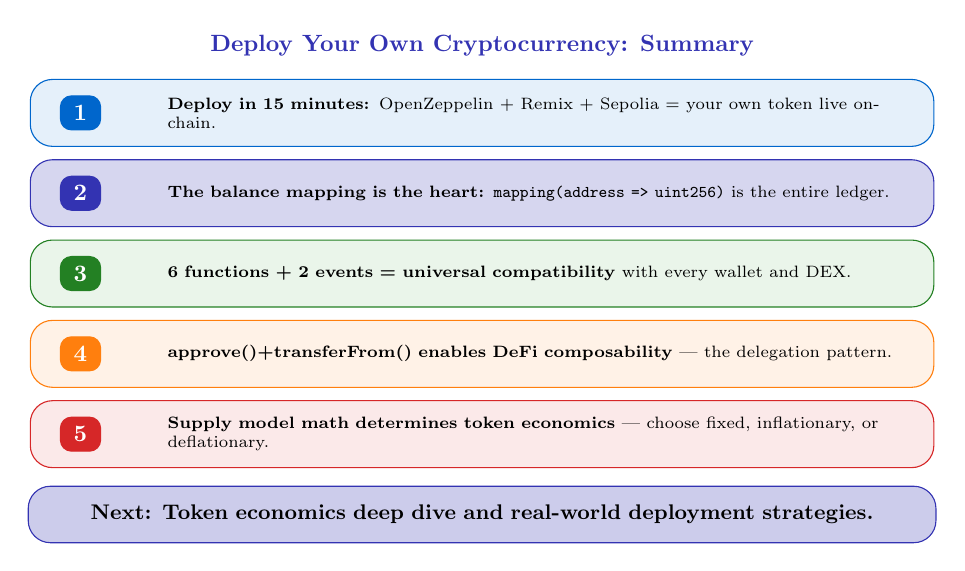
\begin{tikzpicture}[scale=0.85, every node/.style={transform shape}]

\node[font=\normalsize\bfseries, mlpurple] at (0,3.8) {Deploy Your Own Cryptocurrency: Summary};

% === Takeaway 1 (Blue) ===
\node[draw=mlblue, fill=mlblue!10, rounded corners=8pt,
      minimum width=13.5cm, minimum height=1.0cm, inner sep=5pt]
      (t1) at (0,2.8) {};
\node[draw=mlblue, fill=mlblue, text=white, rounded corners=4pt,
      font=\normalsize\bfseries, inner sep=4pt, minimum width=0.6cm]
      at (-6.0,2.8) {1};
\node[font=\scriptsize, text width=11.0cm, align=left] at (0.8,2.8)
     {\textbf{Deploy in 15 minutes:} OpenZeppelin + Remix + Sepolia = your own token live on-chain.};

% === Takeaway 2 (Purple) ===
\node[draw=mlpurple, fill=mllavender4, rounded corners=8pt,
      minimum width=13.5cm, minimum height=1.0cm, inner sep=5pt]
      (t2) at (0,1.6) {};
\node[draw=mlpurple, fill=mlpurple, text=white, rounded corners=4pt,
      font=\normalsize\bfseries, inner sep=4pt, minimum width=0.6cm]
      at (-6.0,1.6) {2};
\node[font=\scriptsize, text width=11.0cm, align=left] at (0.8,1.6)
     {\textbf{The balance mapping is the heart:} \texttt{mapping(address => uint256)} is the entire ledger.};

% === Takeaway 3 (Green) ===
\node[draw=mlgreen!80!black, fill=mlgreen!10, rounded corners=8pt,
      minimum width=13.5cm, minimum height=1.0cm, inner sep=5pt]
      (t3) at (0,0.4) {};
\node[draw=mlgreen!80!black, fill=mlgreen!80!black, text=white, rounded corners=4pt,
      font=\normalsize\bfseries, inner sep=4pt, minimum width=0.6cm]
      at (-6.0,0.4) {3};
\node[font=\scriptsize, text width=11.0cm, align=left] at (0.8,0.4)
     {\textbf{6 functions + 2 events = universal compatibility} with every wallet and DEX.};

% === Takeaway 4 (Orange) ===
\node[draw=mlorange, fill=mlorange!10, rounded corners=8pt,
      minimum width=13.5cm, minimum height=1.0cm, inner sep=5pt]
      (t4) at (0,-0.8) {};
\node[draw=mlorange, fill=mlorange, text=white, rounded corners=4pt,
      font=\normalsize\bfseries, inner sep=4pt, minimum width=0.6cm]
      at (-6.0,-0.8) {4};
\node[font=\scriptsize, text width=11.0cm, align=left] at (0.8,-0.8)
     {\textbf{approve()+transferFrom() enables DeFi composability} --- the delegation pattern.};

% === Takeaway 5 (Red) ===
\node[draw=mlred, fill=mlred!10, rounded corners=8pt,
      minimum width=13.5cm, minimum height=1.0cm, inner sep=5pt]
      (t5) at (0,-2.0) {};
\node[draw=mlred, fill=mlred, text=white, rounded corners=4pt,
      font=\normalsize\bfseries, inner sep=4pt, minimum width=0.6cm]
      at (-6.0,-2.0) {5};
\node[font=\scriptsize, text width=11.0cm, align=left] at (0.8,-2.0)
     {\textbf{Supply model math determines token economics} --- choose fixed, inflationary, or deflationary.};

% === Next lecture teaser ===
\node[draw=mlpurple, fill=mllavender3, rounded corners=8pt,
      font=\small, inner sep=8pt, text width=13cm, align=center]
      at (0,-3.2) {\textbf{Next: Token economics deep dive and real-world deployment strategies.}};

\end{tikzpicture}
\end{center}

\bottomnote{You now have the knowledge to create, deploy, and explain your own ERC-20 token.}
\end{frame}

\end{document}
